\subsubsection{Robuste Regelgüte}
    Wenn gleihzeitig das robuste Nyquist Theorem und die nominelle Spezifikation erfüllt sein sollen spricht man von der \textit{Robusten Regelgüte}.
    
    \begin{equation*}
        \colorboxed{red}{
        \begin{aligned}
            |W_1(\jw)\cdot S(\jw)| + |W_2(\jw)\cdot T(\jw)| < 1\\
            |W_1(\jw)| + |W_2(\jw)\cdot L(\jw)| < |1 + L(\jw)|
        \end{aligned}
        }
    \end{equation*}
    
    \begin{figure}[H]
        \centering
        \includegraphics[width = 0.5\linewidth]{images/03/rob_reggüte.jpeg}
        \caption{Robuste Regelgüte}
        \label{fig:robreg}
    \end{figure}
    
    Um Spezifikationen der Sensitivität und Modellunsicherheit in jedem Fall zu berücksichtigen darf die summierte Länge der beiden roten Pfeile nie länger sein als der blaue Pfeil. Die Beiden Kreise dürfen sich für keine Frequenz berühren/schneiden.
    
    \subsubsection{Approximative Spezifikation}
        Um einen Regler zu finden, der robuste Regelgüte garantiert ist es einfacher wenn man diese nach $L(\jw)$ umformuliert. Dies ist einfach für sehr hohe und sehr tiefe Frequenzen
        
        \textit{tiefe Frequenzen:} $\omega < 0.1\cdot \omega_c \Rightarrow |L(\jw) \gg 1$
        
        Robuste Regelgüte vereinfacht sich zu
        \begin{gather*}
            |W_1(\jw)| + |W_2(\jw)\cdot L(\jw)| < |L(\jw)|\\
            \Rightarrow |L(\jw)| > \frac{|W_1(\jw)|}{1 - |W_2(\jw)|}
        \end{gather*}
        Lösung kann nur existieren falls $|W_2(\jw)| < 1$. 
        
         \textit{Hohe Frequenzen:} $\omega > 10\cdot \omega_c \Rightarrow |L(\jw) \ll 1$
         
        Robuste Regelgüte vereinfacht sich zu
        \begin{gather*}
            |W_1(\jw)| + |W_2(\jw)\cdot L(\jw)| < 1\\
            \Rightarrow |L(\jw)| < \frac{1 - |W_1(\jw)|}{|W_2(\jw)|}
        \end{gather*}
        
        Diese Approximation betrachtet $[0.1\cdot \omega_c, 10\cdot\omega_c]$ nicht. In diesem band ist es vor allem wichtig Stabilität und Robustheit zu garantieren.
        
    \subsubsection{Kompatibilitätsbedingung}
        \textbf{Aus RT1:} Durchtrittsfrequenz $\omega_c$ von $L(\jw)$ soll folgende Bedingungen erfüllen:
        
        \begin{equation*}
            \omega_c = 
            \begin{cases}
                \omega_c > \textnormal{max}\{10\cdot\omega_d, 2\cdot\omega_{\pi^+}\}\\
                \omega_c < \textnormal{min}\{\frac{1}{10}\cdot\omega_n, \frac{1}{10}\cdot \omega_2, \frac{1}{2}\cdot \omega_\tau, \frac{1}{2}\cdot \omega_{\zeta^+}\}
            \end{cases}
        \end{equation*}
        Für konservativere Bedingungen wählt man $5\cdot\omega_{\pi^+}$ und/oder $\frac{1}{5}\cdot \omega_\tau, \frac{1}{5}\cdot \omega_{\zeta^+}$
        
        Dabei sind $\omega_d,\, \omega_{\pi^+},\, \omega_n,\, \omega_2,\, \omega_\tau,\, \omega_{\zeta^+}$ die Frequenzen der Störung, des schnellsten instabilen Poles von $L(s)$, des Rauschens, von $|W_2(\jw_2)|=1$, der Totzeit und der langsamsten nicht-minphasigen NST.
        
        Die Frequenz $\omega_1$ bei $|W_1(\jw_1)| = 1$ muss kleiner sein als $\omega_2$, sodass $\omega_c$ genügend Marge hat. Zudem muss $\omega_1$ aber schneller sein als die untere Schranke für $\omega_c$. Man wählt als erste Schätzung
        \begin{equation*}
            \omega_1 \approx \textnormal{max}\{10\cdot\omega_d, 2\cdot\omega_{\pi^+}\}
        \end{equation*}
        
        Zusätzlich muss $\omega_1$ grösser gewählt werden, je grösser die gewünschte Phasenreserve $\varphi$ sein soll. Dies kann mit der Magnitude der Sensitivität bei $\omega_c$ interpretiert werden:
        \begin{equation*}
            |S(\jw)| = \frac{1}{|1+L(\jw_c)|}= \frac{1}{|1+1\cdot e^{-j(\pi-\varphi)}|} = \frac{1}{\sqrt{2}\cdot\sqrt{1-\cos{\varphi}}}
        \end{equation*}
        
        In der Regel nimmt $|S(\jw)|$ mit ansteigender Frequenz zu und schneidet die 0 dB Linie einmalig.
        
        \begin{figure}[H]
            \centering
            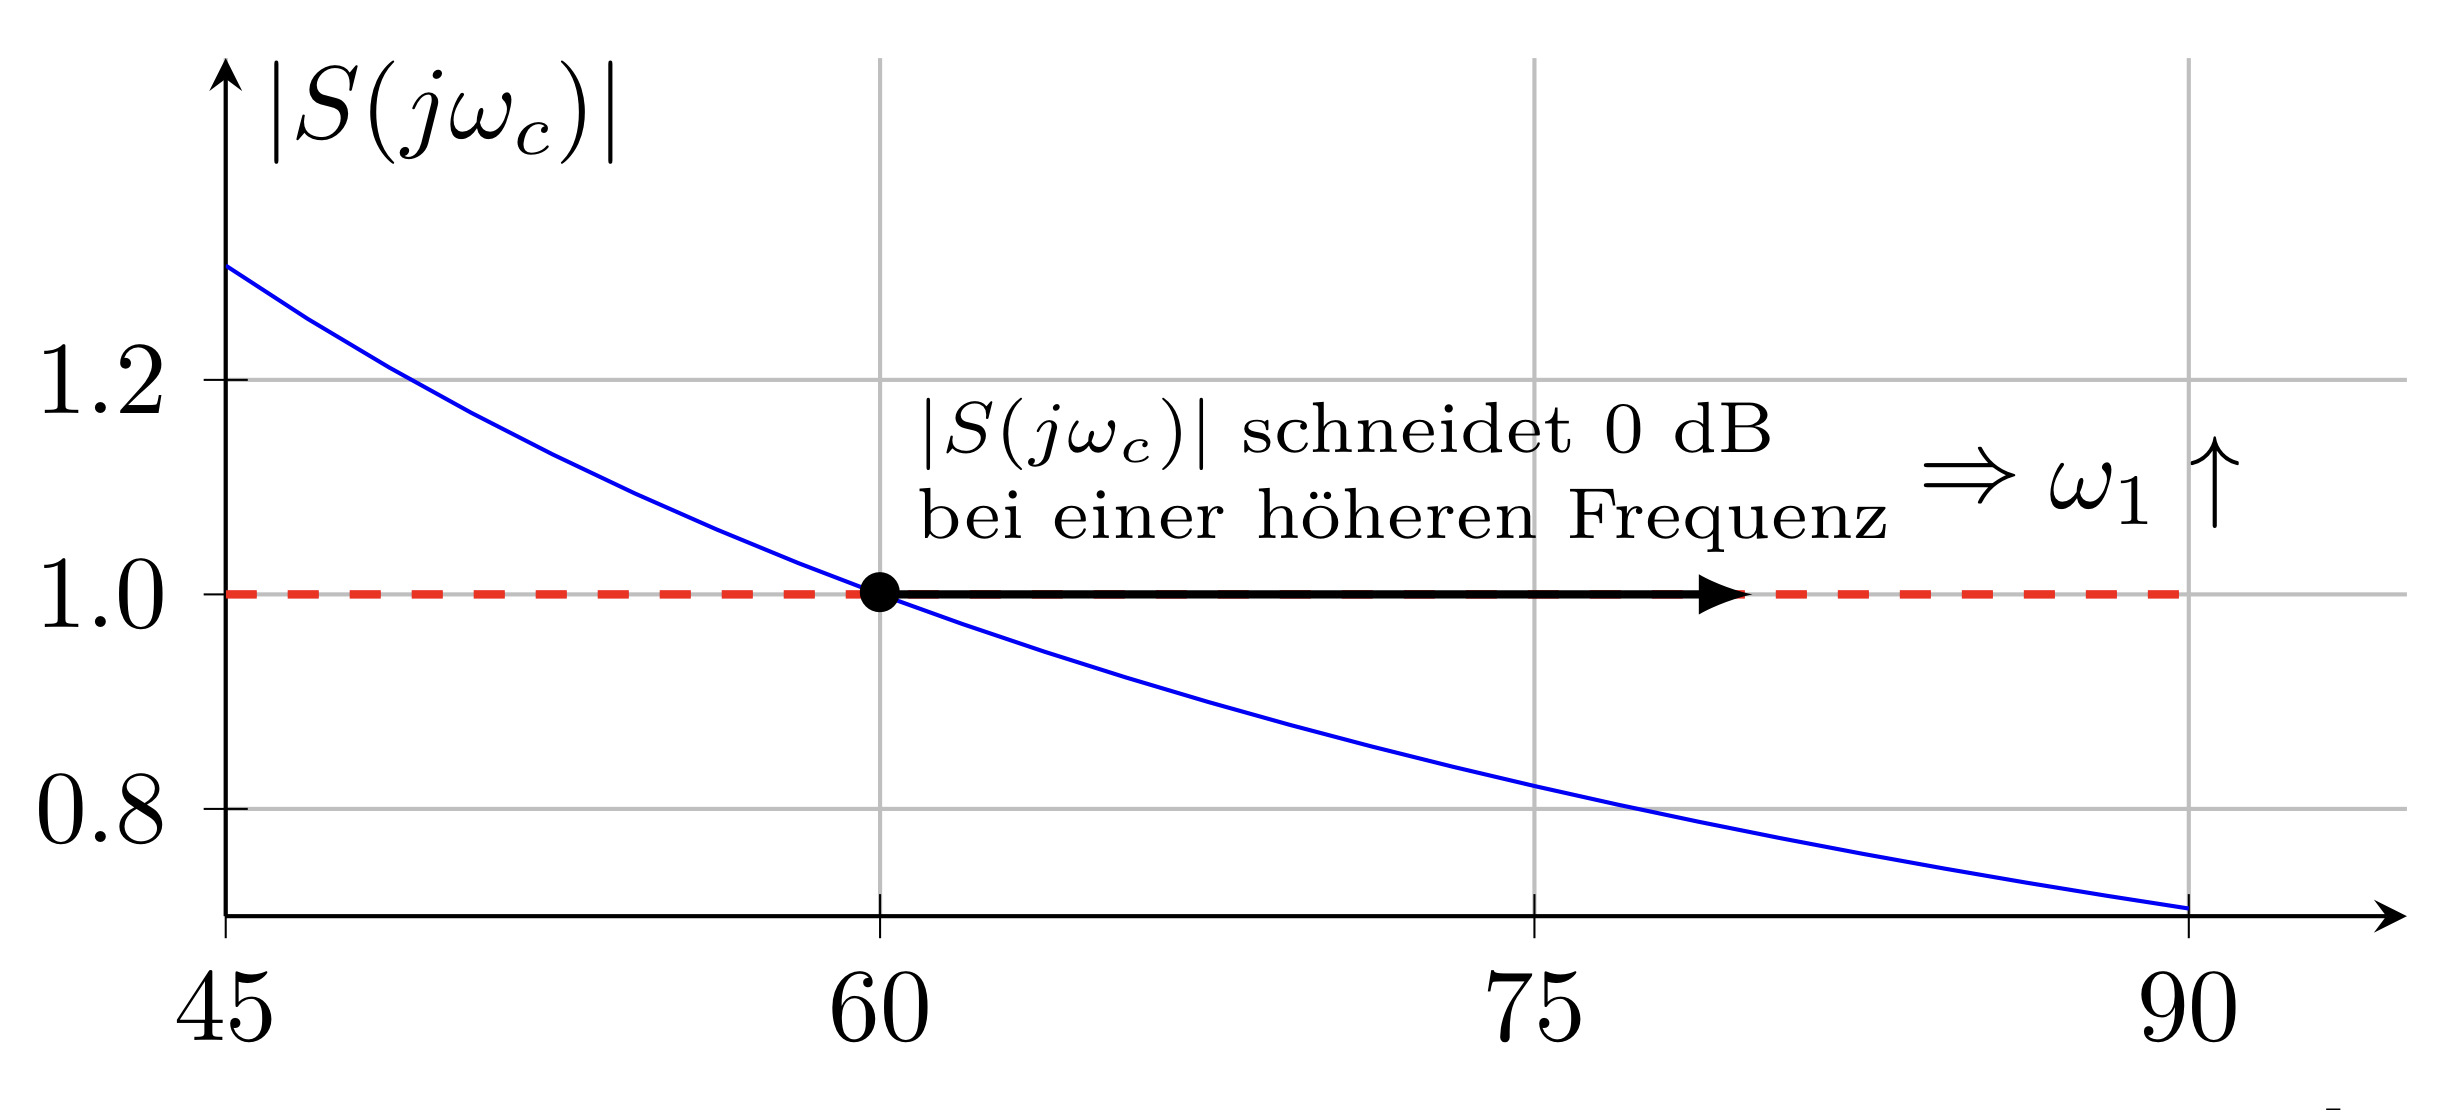
\includegraphics[width = 0.5\linewidth]{images/03/phasemargin.jpeg}
            \caption{$|S(\jw_c)|$ als funktion von $\varphi$}
            \label{fig:pmarg}
        \end{figure}
        
        In Abb. \ref{fig:pmarg} ist die Magnitude der Sensitivität als Funktion der Phasenreserve dargestellt. Magnitude wird kleiner, je grösser die gewünschte Phasenreserve ist. Dh, die Sensitivität muss die 0 dB Linie bei einer höheren Frequenz schneiden, je grösser $\varphi$ sein soll. $\Rightarrow$ $\omega_1$ muss höher spezifiziert werden.
        
        Man kann auch mit Abb. \ref{fig:robreg} argumentieren. $|W_1(\jw)|$ wird bis zu $\omega_1$ grösser als 1 sein. Je grösser $|W_1(\jw)|$ ist, desto grösser muss $\varphi$ sein, da ansonst $L(\jw)$ ind den Kreis von $|W_1(\jw)|$ eintreten würde.
        
        \begin{figure}[H]
            \centering
            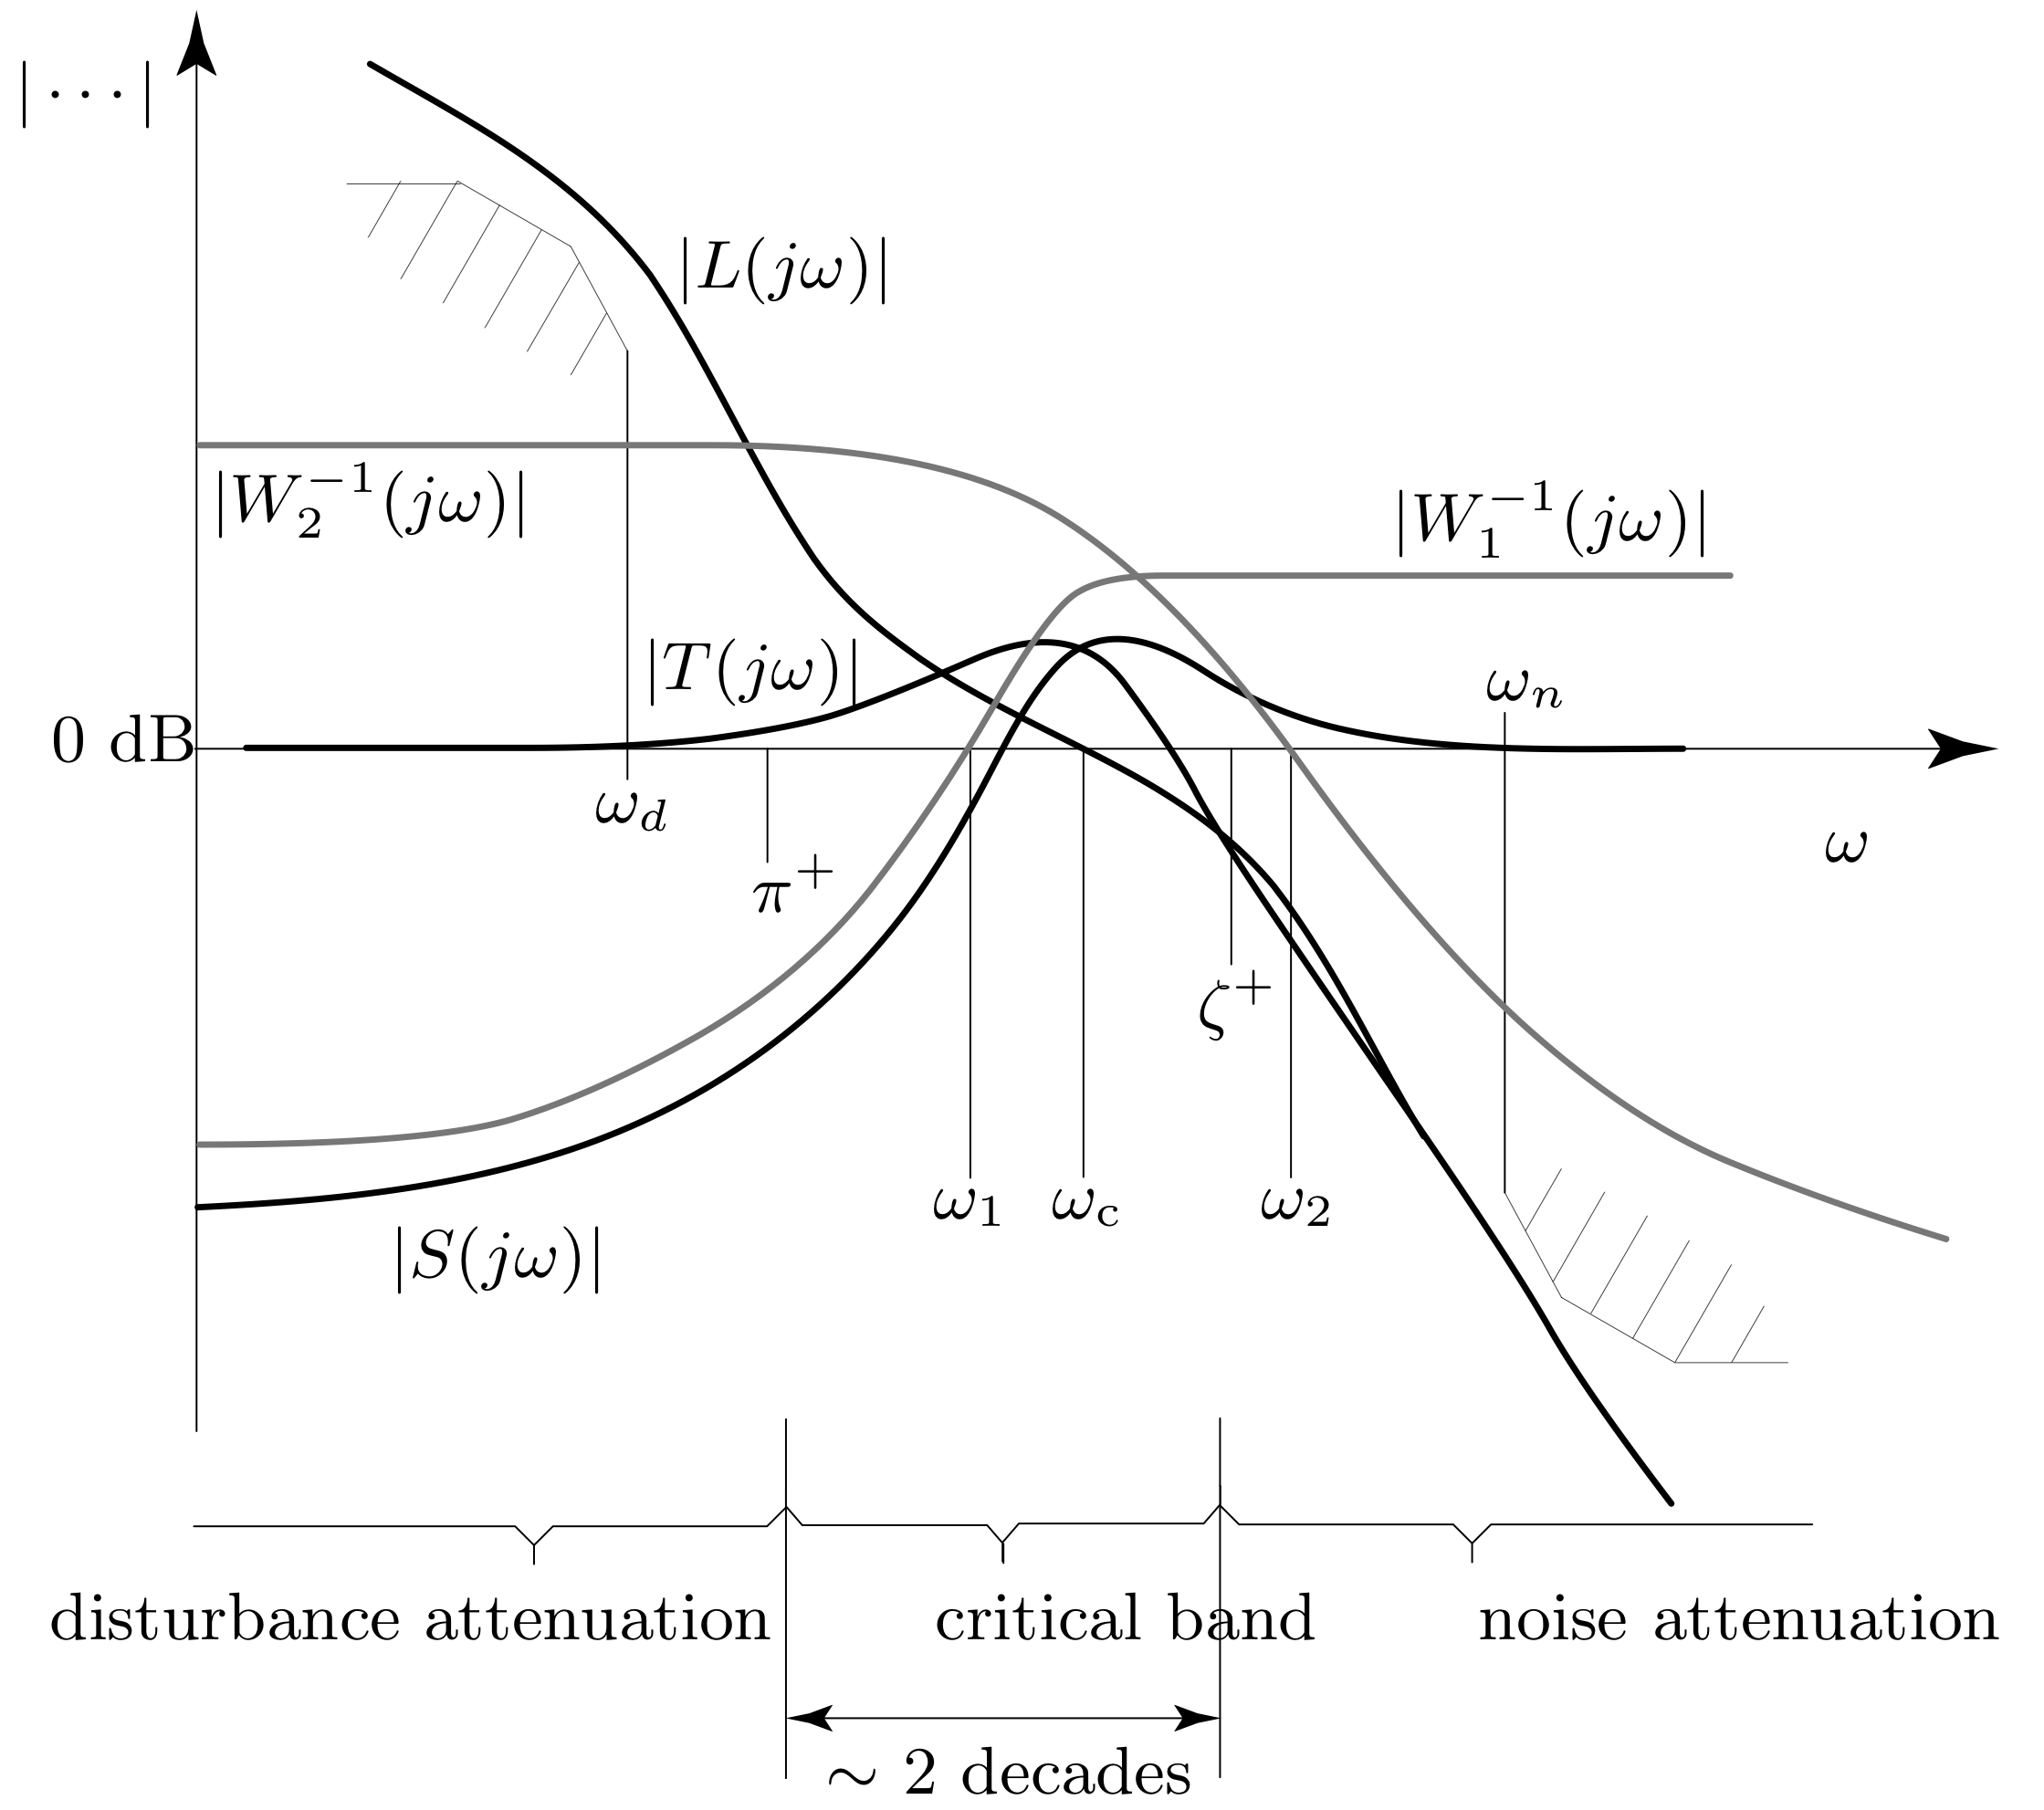
\includegraphics[width = 0.6\linewidth]{images/03/summary_specifications.jpeg}
            \caption{Zusammenfassung aller Bedingungen und Spezifikationen}
        \end{figure}